\documentclass{proposal}

\title{BrainSign:  Recognizing American Sign Language from Brain Signals}

\begin{document}
\maketitle

\noindent{\bf C. Project Description}\\

\section{Direct Brain Interfaces}

Nearly two million people in the US alone suffer from severe motor disabilities that render them incapable of communicating with the outside world \cite{ficke1992ddp, NABMRR1992, murray1997gmd, carter1997rmn}. Direct brain interfaces (DBIs) measure neural activation to provide a communication and control channel that is independent of muscle movement. To date, the best performance for a DBI communication system is 68 bit per minute (just over 8 characters per minute) \cite{gao2003bbe}, a rate attained using the Steady-State Visual Evoked Potential (SSVEP). While the progress made so far is notable, it pales in comparison to the transmission rates attained by signers and speakers (175-200 words per minute).

\section{Recognizing Imagined Sign from fMRI} % and EEG}

We hypothesize that DBI communication rates can be increased by recognizing phrases of American Sign Language (ASL) from the motor cortex.  Previous research suggests that \textit{imagined} movements are expected to produce neural activations similar, though lesser in magnitude, to \textit{executed} movements \cite{beisteiner1995mrm,pfurtscheller1997mia, lang1996eam,lotze1999aac}. For people who are ``locked-in,'' such a system could significantly improve their ability to communicate.

Imagine a person with a progressive muscular disease such as ALS.  As the symptoms worsen, he learns useful signs or phrases of sign (see Figure \ref{fig:brainsign}).When finally locked-in and in need of a DBI, he then imagines or attempts to produce these ASL phrases. BrainSign, our recognition system, then recognizes these signs and displays the appropriate English translation for the user's communication partners.

%\begin{figure}[h]
%\centering
%\fbox{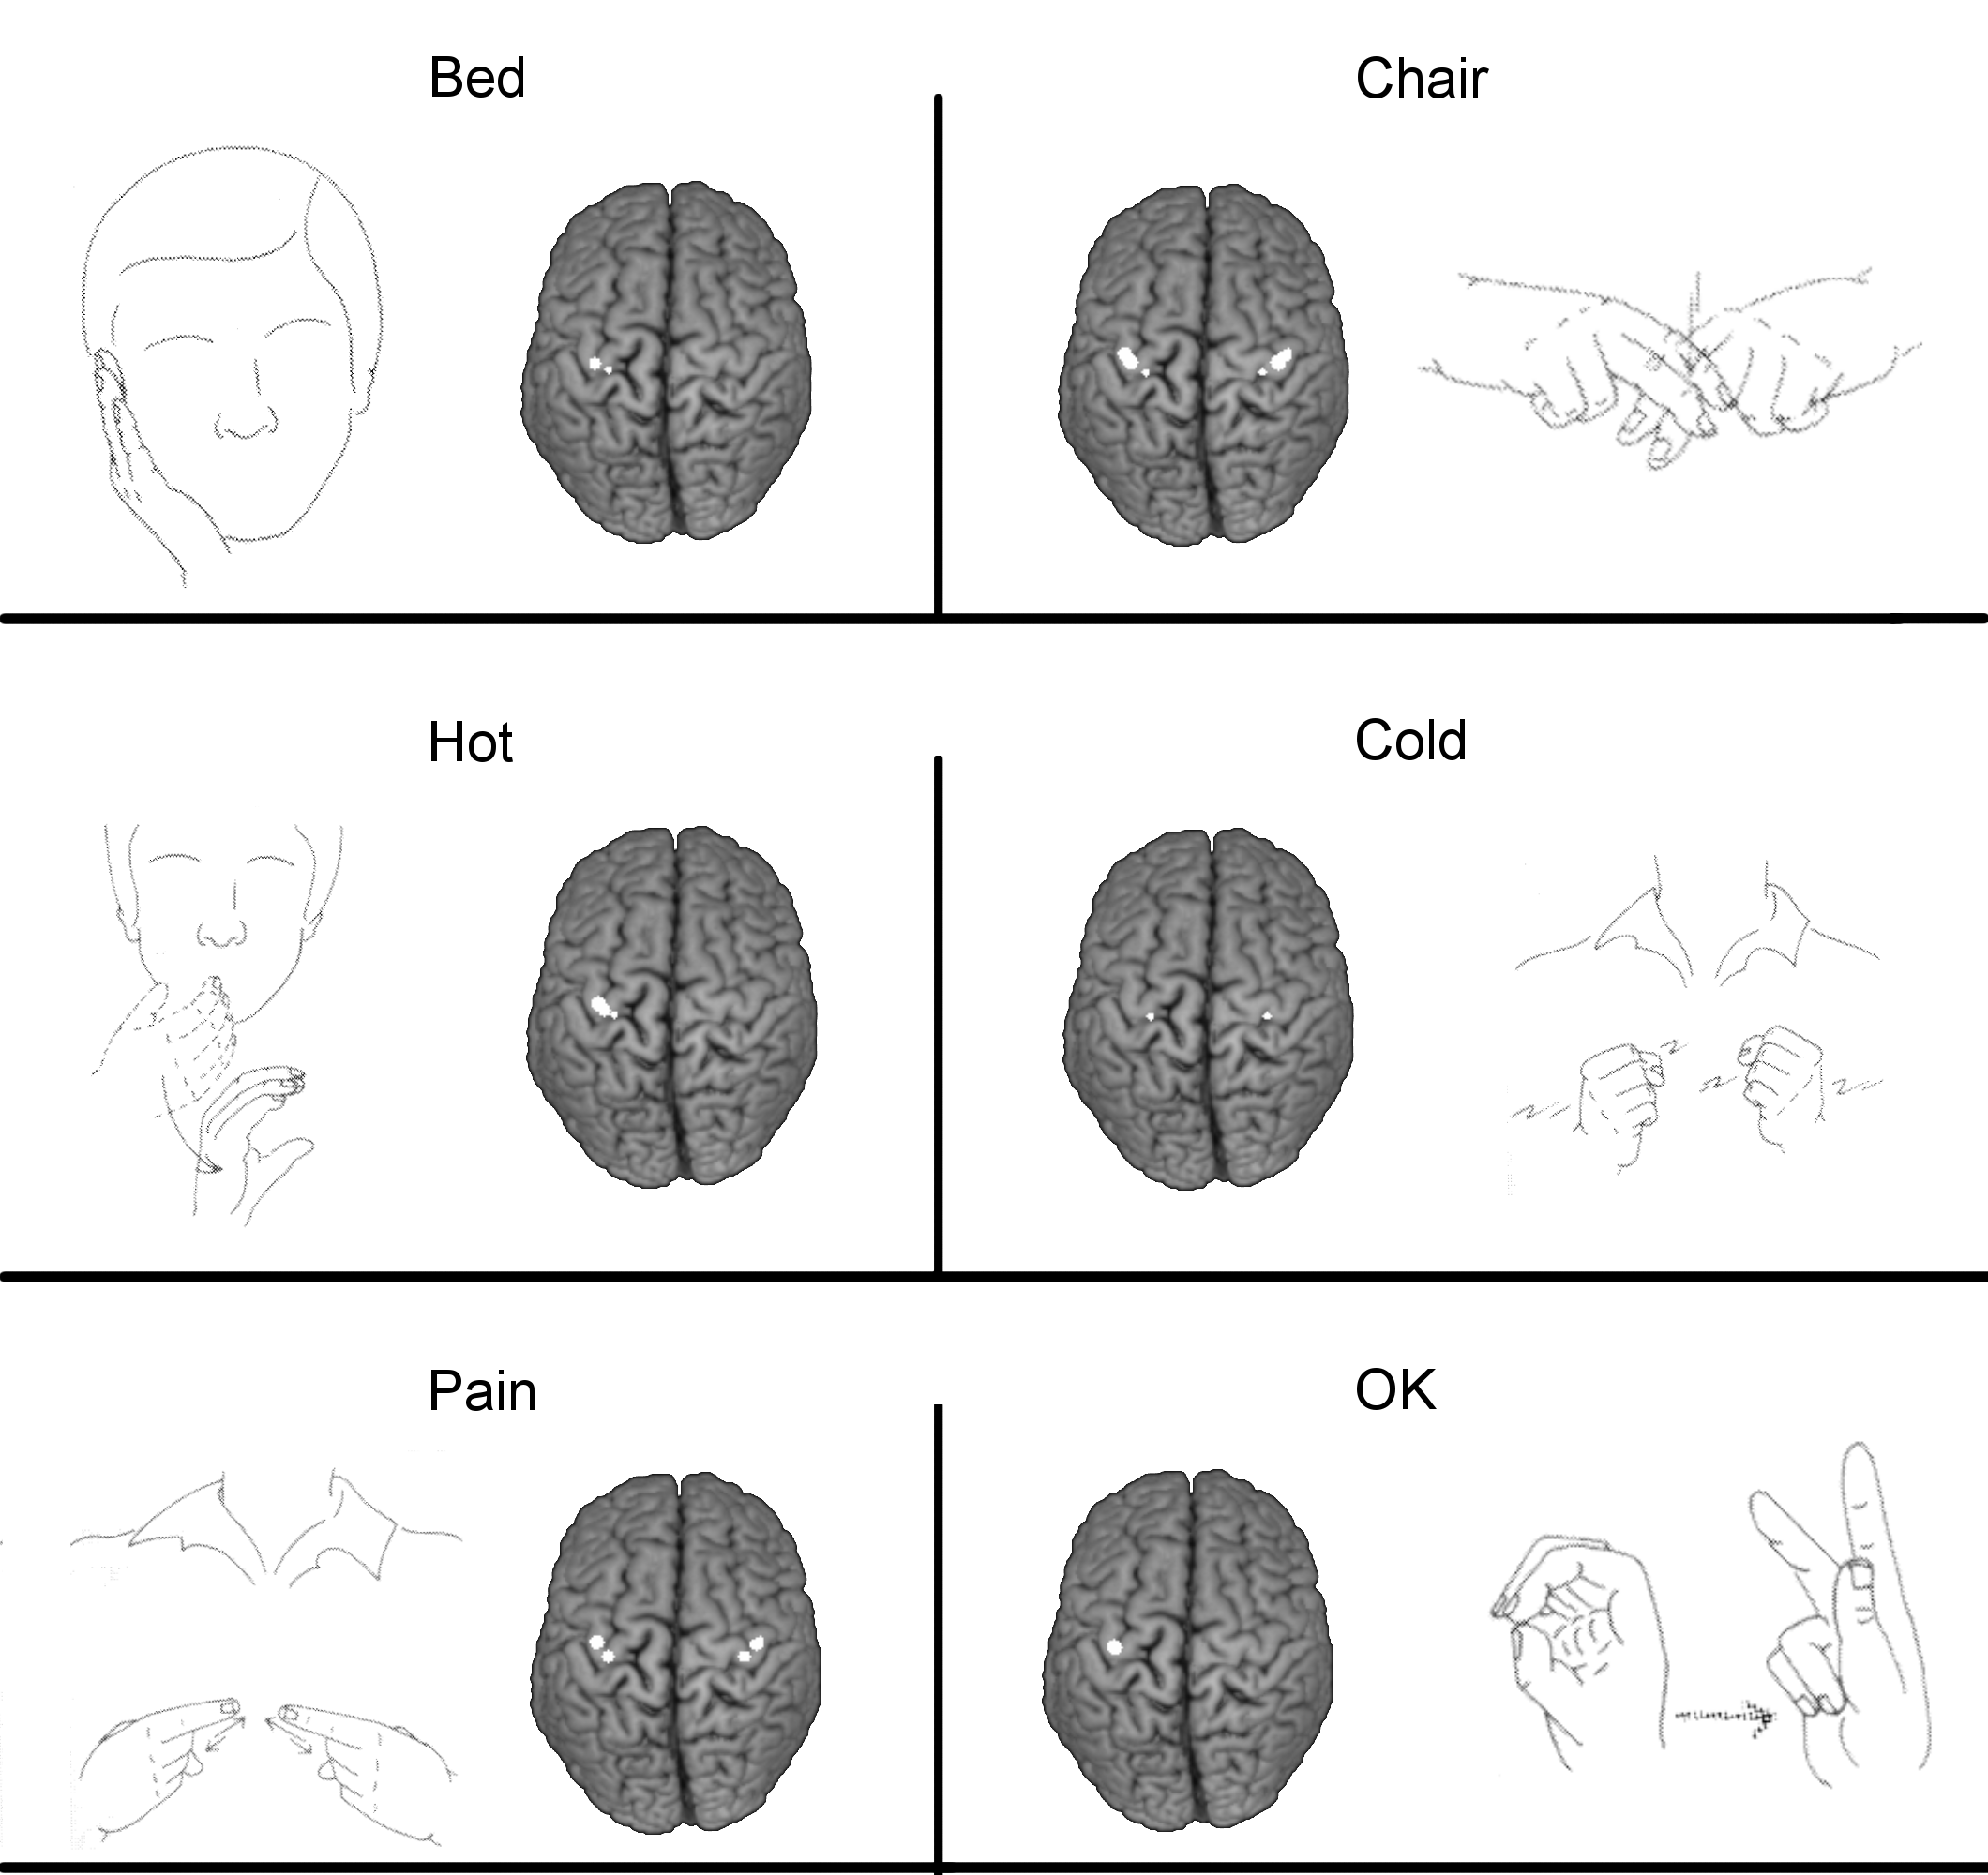
\includegraphics[width=120mm]{all_vs.png}}
%\caption{Three sets of paired signs where we expect the activation in the motor cortex to be sufficiently distinct for recognition. Regions of activation due to sign are shown in white. The brain images were produced by MRIcron, available at http://www.mricro.com/mricron.}
%\label{fig:brainsign}
%\end{figure}

\begin{figure}[ht]
\begin{minipage}[t]{120mm}
\begin{center}
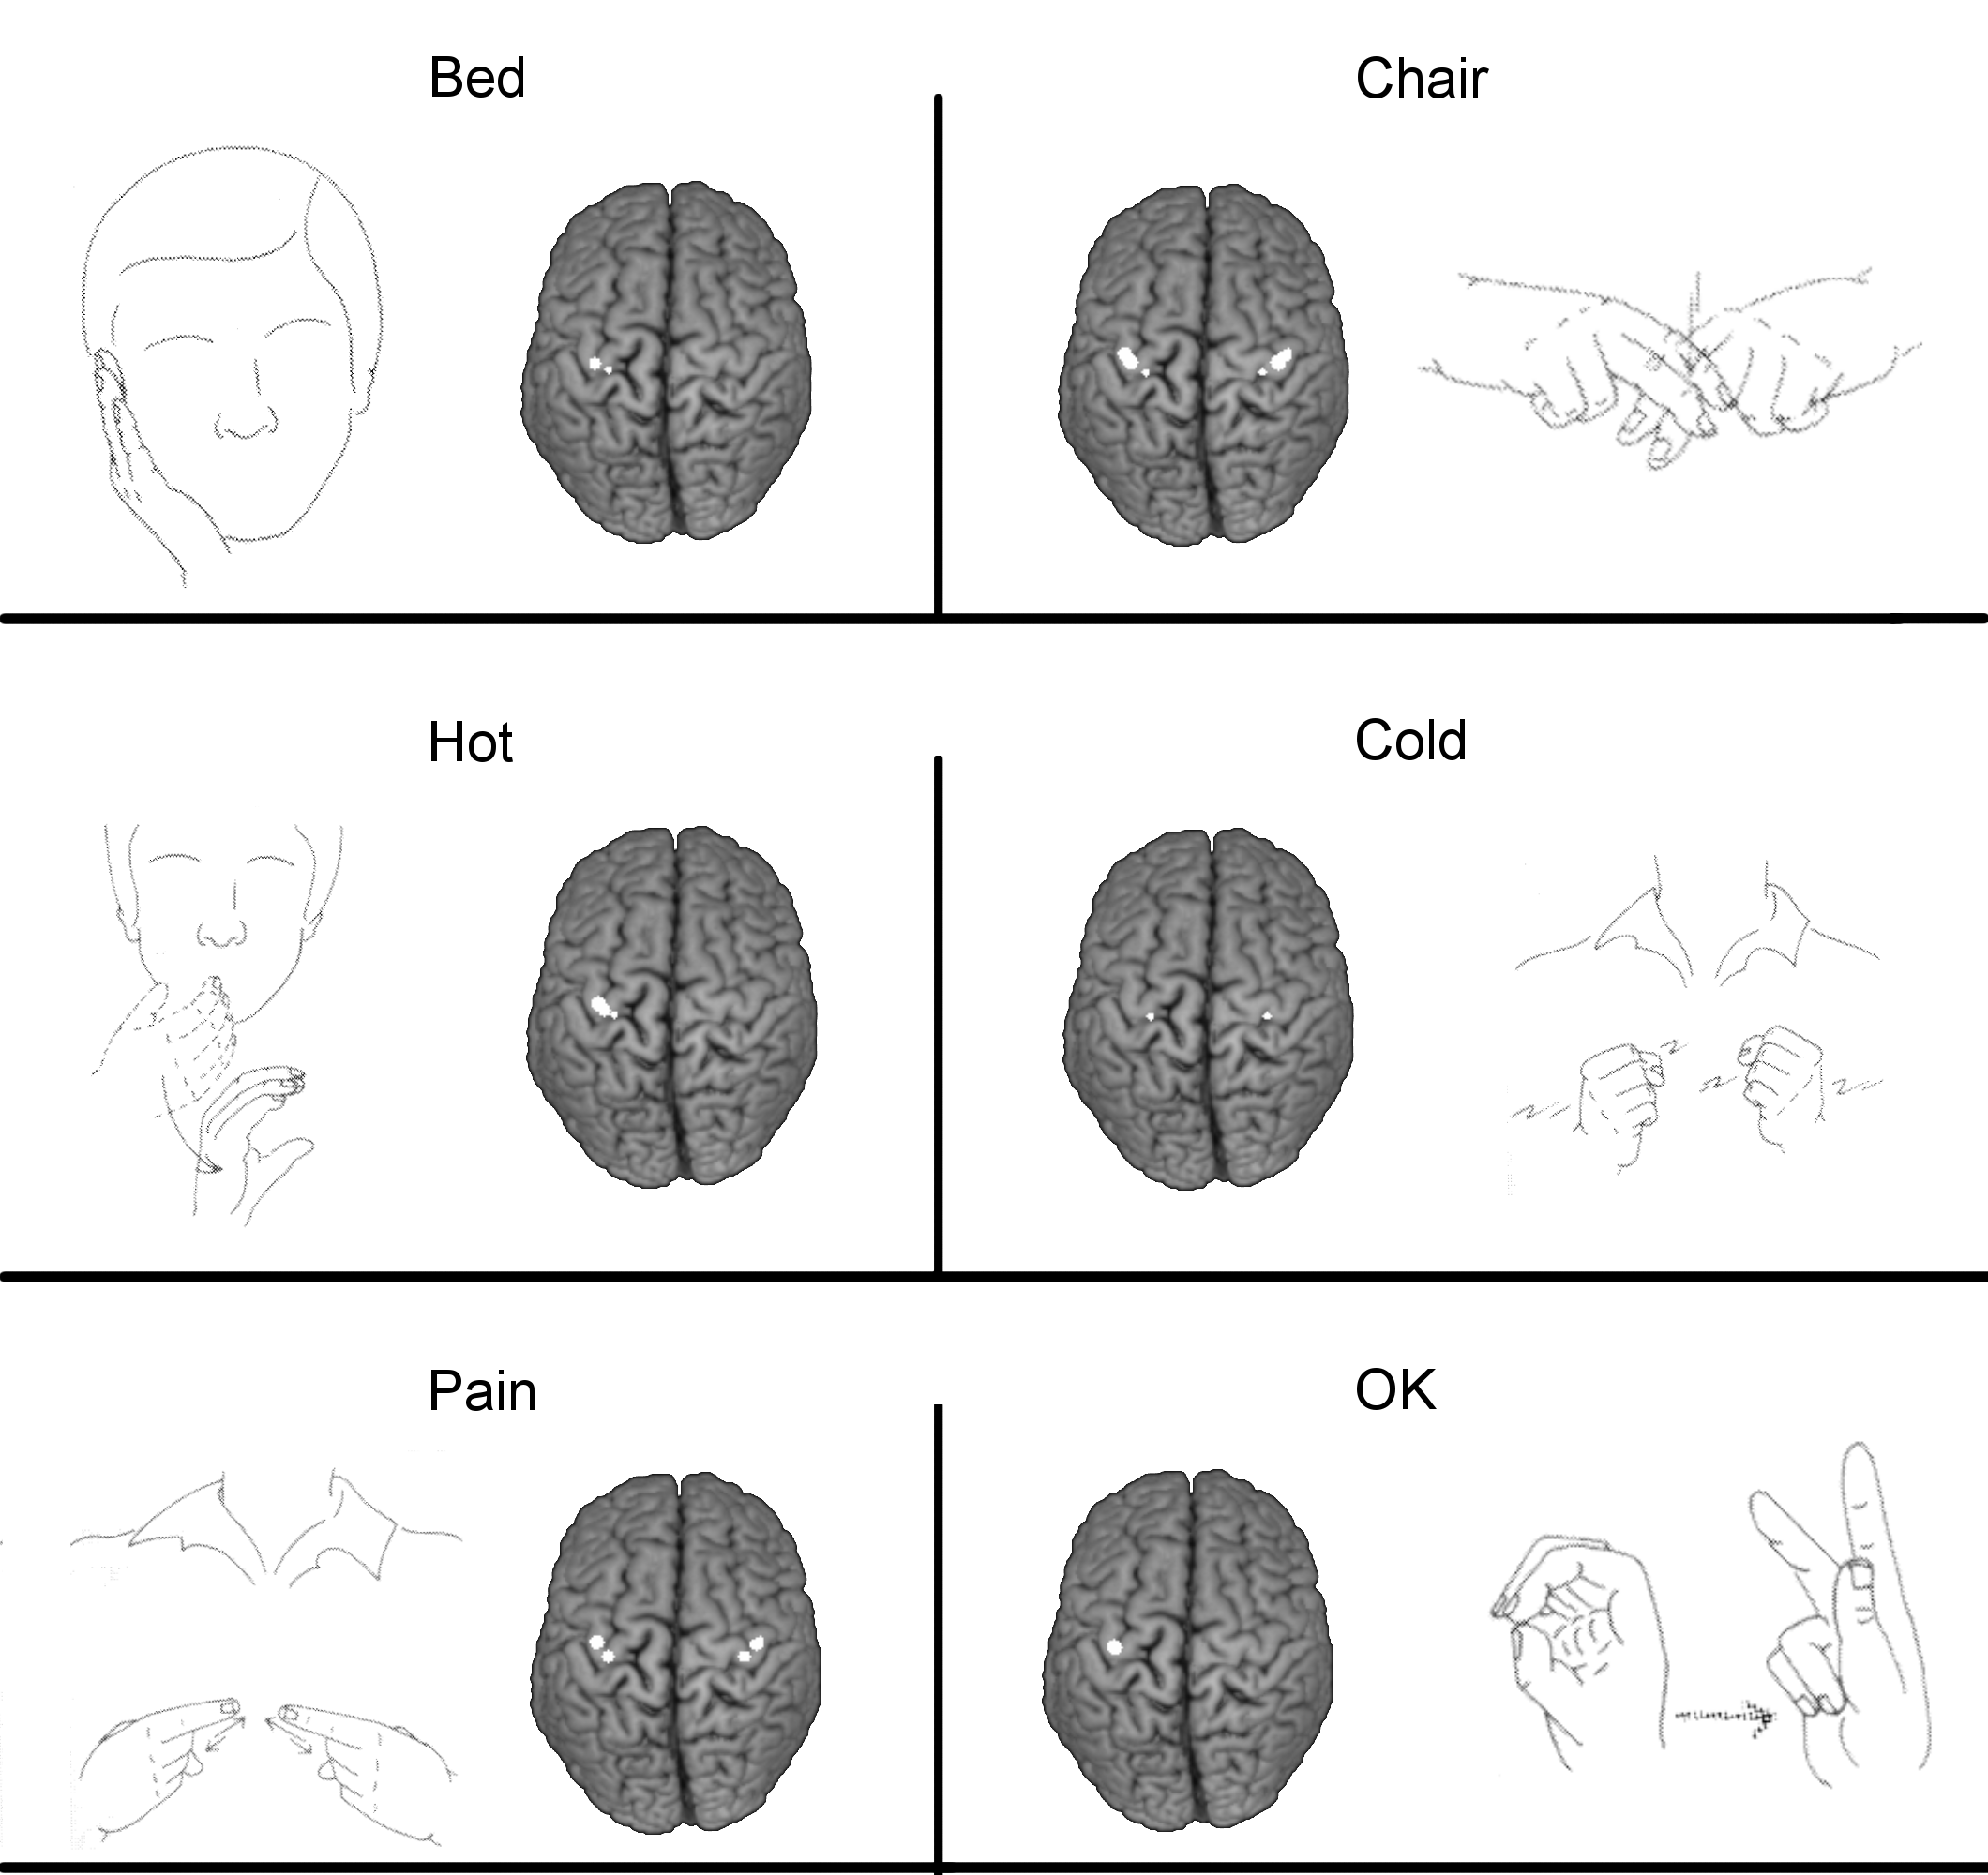
\includegraphics[width=120mm,clip]{all_vs.png}
\end{center}
\end{minipage}
\hfill
\begin{minipage}[t]{35mm}
\begin{center}
\includegraphics[width=35mm]{BedHotIPain_time_slices.png}
\end{center}
\end{minipage}
\caption{\label{fig:brainsign} At left, three sets of paired signs where we expect motor cortex activation to be sufficiently distinct for recognition. Regions of activation due to sign are shown in white. At right, time increasing from top to bottom, temporal progression of activation on the motor cortex strip during signing of ``Bed Hot I Pain.'' Brighter white indicates higher activation. The brain images were produced by MRIcron, available at http://www.mricro.com/mricron.}
\end{figure}


Vocal speech involves muscles (tongue, larynx, etc.) in a relatively small region of the motor cortex, and phonemes are relatively indistinct from each other at the spatial and temporal scales currently detectable with brain imagers; however, signs are constructed using much coarser muscle movements (shoulders, arms, hands, fingers, face, etc.) and often vastly differ from each other: one versus two handed production, static versus sweeping arm postures, fixed versus dynamic finger poses, and symmetry of left and right hand shapes.  Figure \ref{fig:brainsign} demonstrates pairs of signs where we expect
%both
fMRI activation
%and event related potentials (ERPs)
to be distinct.  The simplest version of BrainSign would be an interface where the user attempts to produce one of two signs (e.g. ``cold'' or ``hot'') in response to a question.  The user would simply imagine producing that sign repeatedly until a timeout appropriate for the sensing technology.  A more sophisticated interface would allow the user to select from a series of distinct signs.  Note that the expected
activations %ERPs
for the six signs in Figure \ref{fig:brainsign} are distinct and represent potential needs for a locked-in user (i.e. I'm ``hot'' or ``cold,'' I want to go to ``bed'' or go to my ``chair,'' I am in ``pain'' or I'm ``OK'').  Such an interface may allow the user to communicate more quickly; however, the fastest interface would be a system that distinguishes entire phrases of sign. Just as with a foreign language phrasebook, signed phrases could be chosen for their utility and their likelihood of being understood (in this case, by the DBI).

%Current brain imaging techniques, such as fMRI, have good spatial resolution at a cost of temporal resolution, while EEG has good temporal and poor spatial characteristics.  With these constraints, how can signed phrases be recognized?  

For recognizing ASL phrases with fMRI, our proof of concept task, one can think of the brain as a slowly refreshing display where the consecutive images bleed into each other.  Imagine watercolor painting with disappearing ink.  The portions of the canvas the painter brushes lightly have a small change in color. Places where the painter dwells absorb more ink, become darker, and take more time to disappear.  A snapshot of the canvas, taken at the right time, could reveal the painter's intended image. In our case, a signed phrase such as ``Bed hot, I pain'' corresponds to the major posture changes (right hand/wrist/elbow/shoulder; right index finger/thumb/wrist; right fingers/wrist/elbow; right and left wrists).  The resulting ``painting'' would show a large lightly colored region reflecting the grosser movements to get the hands in position, a dark region reflecting the effort of the fingers of the right hand, and two symmetric dark regions showing the repeated twisting of the wrists for ``pain.''

Continuing the analogy, a snapshot taken at the wrong time could lead the viewer astray; however, a movie showing the progression of strokes would be easier for the viewer to understand.  We hypothesize that such signed sequences are recognizable from a continuous stream of brain imaging.  Specifically, we will combine hidden Markov models (HMMs),
%we might consider mentioning conditional random fields or max-margin markov networks here as they are probably far better for this classification task
which Starner has shown to be effective at recognizing phrases of sign \cite{starner1998rta}, with Bobick's Temporal Templates \cite{bobick2001rhm}, which identified user actions in video through snapshots as described above. In all our experiments we will report accuracies for both the continuous and isolated recognition tasks using the ISO standards developed from the speech recognition domain.

%While recognizing a natural language directly from the brain would be a breakthrough along several dimensions, fMRI is not practical for everyday communication.  Instead, we will focus on EEG for that task.  Unfortunately, EEG's spatial resolution will not be able to differentiate finger motions.  However, we suspect that EEG will be able to differentiate between signs that are (imagined to be) produced with the left or right hands.  Carefully constructed phrases should be distinguishable simply by the time sequence of activation patterns of the right and left hands.  Of course, if higher spatial resolution proves possible, then a wider range of phrases will be possible.  If, however, EEG can not distinguish between left and right hands, we may have users imagine moving their left foot as if it was the left hand.  This technique will preserve the intuitive mapping of using real sign language while providing better discrimination.  



\section{Related Work}

To date there has been little work towards recognizing signs and sign phrases using brain signals. Previous electroencephalography (EEG) work has shown discriminative ability between different appendage movements (left/right hand/foot). Previous studies with brain imaging of sign language have focused on specific linguistic properties (presence of meaning, semantic ambiguity, nouns versus verbs, motor iconicity, and locative classifiers) \cite{supp2005_smr, tranel2005_env, lee2006_mme, dehaene1995_eec, hjorth1975_oie, perrin1988_sss, corina2003_llb, emmorey2004_mis, emmorey_broca_region_2006}. New evidence suggests that fMRI can capture movements of interest for discriminating ASL. \cite{rao1996rbf} observed a linear relationship between movement rate and fMRI activation , and \cite{kim1997ltr} showed that spatially proximate neural events occuring at least 4 seconds apart are separable in fMRI. This suggests that we may use the fMRI time course for discriminating between long-duration ($\geq$ 4 s) events.

%For the EEG-based BrainSign system, we will boost the spatial resolution of the EEG using fMRI. Recent methods generally identify spatial locations of EEG sources by using spatial information from fMRI activations. Mapping scalp-recorded EEG to three-dimensional source locations is an ill-posed problem, but constraining mappings by fMRI prior knowledge greatly makes the problem well-posed. \cite{im2006tcm} developed a method for weighting fMRI functional priors according to how well the the fMRI matches spatial activation inferred from EEG alone. Additional research by \cite{ahlfors1999sac} uses fMRI to electric dipoles, while \cite{wagner2000fcd} demonstrated fMRI-constrained cortical current density estimation. The most promising for our work may be \cite{dale2000dsp}'s demonstration that fMRI recorded during stimulus presentation can be incorporated into EEG source localization, using Bayesian statistics and an approximation electrical activity/hemodynamic response dependency.

%\subsection{Novel Experiment Design}
%To accomplish our goals, we invoke a paradigm shift in fMRI analysis. We consider gesture differentiation using time series of fMRI slices. Similar to response to a blocked-task, but instead of accomplishing longer activation duration via repeated activation using the same stimulus/activity, we consider longer activation duration via a stimulus/activity spanning a long time window. One example of such a ``long'' activity is a sequence of gestures, rather than a single gesture. This differs from classical blocked-task, where activation builds in certain areas from repeated application of a stimulus that affects a certain cerebral region. In this case, we may be stimulating different cerebral regions with each atom of the sequence, but recognition still becomes statistically feasible because of evidence provided by single-trial fMRI work \cite{buckner1996dca}. An important question to answer is whether spatiotemporal fMRI activation maps of such temporal uncertainty provide well-separated events in the statistical identifiability sense (as testable by machine learning methods).


\section{Justification for SGER Support}

This is the first project to precisely focus on motor differences in fMRI activation patterns during signing. To our knowledge, no one has yet analyzed the fMRI time course of sign language phrases for ASL recognition.
%Using EEG for ASL recognition is uncharted territory with potentially extraordinary rewards for disabled populations.
Our proposed work on identifying motion patterns using fMRI
%and later EEG
data of the motion patterns also is new, and any discoveries in this area can contribute fundamentally towards a deeper understanding of motor planning/cognition. The research's impact is to offer the target populations unmatched levels of communication with the world.
%Additionally, our use of the proposed long-duration-activity fMRI experiment design will lay the groundwork for other researchers to apply this design to countless other experiments to prove statistical correlations for new stimuli/activites with high statistical power.


\section{Research Approach and Objectives}

Our approach strives to verify the signal discriminability of fMRI
%and EEG
for multiple classes of motion categories, including single signs, sign phrases, and motion patterns, both for executed and imagined movement. All of the experiments will be performed 3 times so that they can be iteratively refined, and each experiment will be 3 hours long. Prior to imaging
%/recording
subjects during the imagined movement experiments, we will verify that the subjects' imagined movements produce motor cortex activation; this verification will be done using EEG focused at the motor cortex with electromyography (EMG) verifying that no actual movement is occurring.

To minimize head movement during signing on an fMRI bed, we will follow \cite{culham2003vgg} and apply arm braces to restrict shoulder and elbow movement. In order to correct any movement artifacts picked up in the fMRI, we will make use of machine learning methods for movement artifact removal \cite{mckeown1998afd}.

We will record subjects performing three experiments: (1) signing individual signs in single trial experiments, (2) signing similarly selected set of phrases, and (3) producing particular patterns of motion (e.g. for a \textit{rotation} pattern, using hand rotation or foot rotation)

The individual signs selected will span a key set of properties (left/right hand only, coarse/fine movement, individual finger movements) to maximize the utility of our analysis. The use of single trials in experiment (1) is justified by \cite{buckner1996dca}, who showed that single trial fMRI recording provides sufficient statistical power for discriminating stimuli. Since phrases consist of multiple signs, we expect substantially greater discrimination likelihood for experiment (2). Notably, activity duration for phrases likely will be between 5 - 10 seconds, and so by the painting analogy we expect that the longer duration of the activity will increase sign phrase discriminability. Experiment (3), has not yet been studied and serves as a novel contribution to motor planning cognition. After training subjects to verify ability to produce the same motion patterns with their hands and feet, subjects will this last experiment and and our analysis will apply machine learning algorithms to detect patterns in the fMRI time courses for particular motion patterns.


%%% NEW FORWARD LOOKING EEG SNIPPET
If we observe positive results in discriminating ASL from the fMRI, we will extend the initial study to EEG as well. A sizeable body of previous work using Bayesian methods suggests that data obtained from fMRI and EEG can be fused to recover neural activation data with both high spatial and high temporal resolution \cite{im2006tcm, ahlfors1999sac, wagner2000fcd, dale2000dsp}. Because of the high temporal resolution of EEG and the high spatial resolution of fMRI, a system combining the two sensing modalities can make BrainSign a portable direct-brain interface that accurately classifies sign phrases from EEG.
%%%

%After exploring the spatiotemporal activation patterns in the fMRI, we will record EEG while subjects perform the three experiments. Our analysis will employ functional priors obtained from the fMRI experiment data, facilitating source localization of the scalp potentials to three-dimensional regions in the brain. We then will apply HMM and temporal template models to recognize signs and phrases. The result will be the first direct-brain interface that classifies sign phrases from EEG.

Our objectives are two-fold:
\begin{enumerate}
\item \textit{Characterize the discriminability of sign language using fMRI data} - Discover the extent to which single ASL gestures of varying complexity can be discriminated from fMRI. We will characterize the extent to which patterns in fMRI time course are common to particular large motion patterns independent of the appendage used (e.g. left hand vs right foot).
\item \textit{Gesture discrimination using fMRI}
%-informed EEG source localization
 - Conduct the first known analysis of ASL recognition using
%EEG
fMRI, allowing future work that recognizes ASL from fMRI-informed EEG.
%, using functional priors obtained from the fMRI results to conduct constrained source localization of the EEG.
Apply the analysis to create the first known portable system that recognizes ASL from brain signals.
\end{enumerate}

\section{Expected Significance and Impact on the Field}
This work will make large contributions towards the field of direct-brain interfaces. It will constitute the first DBI that provides very high information transmission rates, because the number of possible signs that may be expressed is not necessarily bounded. The proposed research lays the groundwork for developing high spatiotemporal resolution pattern recognition for DBIs, and the forward-looking EEG work can benefit the research community greatly by offering a rich example of a synthesis of EEG pattern recognition and fMRI pattern recognition methods.

Our work also may contribute considerably towards cognitive neuroscience, serving as the first comprehensive study of spatially co-located, cognitively orthogonal motor tasks. Some previous work has considered neural activation trends with respect to rate of motor movement \cite{rao1996rbf}, but there has not been a thorough analysis of varying combination of muscles with varying magnitudes, speed, and motion patterns. Our analysis will lead to a more detailed understanding of motor planning and motor activations during sign language and many other motorically similar actions. The additional study of identifying neural activation patterns for particular classes of motion patterns will encourage further spatial pattern analysis. The use of long-duration activity recording provides a model that can be applied to countless other experiments for increased statistical power.


\section{Broader Impacts}

This work can produce a DBI for many people that work in mobility-restricted environments, increasing their communication bandwidth by a wide margin as compared to the current best information capacity of a DBI (68 bits/min previously attained using SSVEP \cite{gao2003bbe}). We will make our data available via a public database so that others can improve on our results using their algorithms. This data further could be used by cognitive neuroscientists and linguists to explore previously unknown signals correlated with language production. The collaboration entailed by this project will encourage cross-pollination of ideas between undergraduates and graduates from fields spanning cognitive neuroscience, intelligent systems, statistics, and control systems design.


\section{Relation to Longer-term Goals of PI}

\section{Most Relevant Results from Prior NSF Support}

Starner's NSF Telesign grant developed the Segmentally Based HMM-based sign language recognizer that will be adapted for this work.


\section{Plan of Work}

Yes


\section{Educational Activities}

The graduate students involved will learn about sign language, neuroscience, and biomedical imaging. Including an undergraduate in the project introduces them to cutting edge research; empirically, undergraduate participation in research significantly increases their chances of pursuing graduate studies \cite{hathaway2002rur}. We will hold a lecture at the Atlanta Area School for the Deaf high school program, explaining our methods for recognizing ASL in the brain using fMRI and EEG.


\bibliography{bib}
\bibliographystyle{ieeetr}


\end{document}
